\documentclass[11pt]{article}
\usepackage[letterpaper,margin=0.82in]{geometry}
\usepackage{amsmath,amssymb,amsthm,mathtools}
\usepackage{graphicx}
\usepackage{xcolor}
\usepackage[hidelinks]{hyperref}
\usepackage{microtype}

\newtheorem{theorem}{Theorem}
\newtheorem{lemma}[theorem]{Lemma}
\newtheorem{corollary}[theorem]{Corollary}
\theoremstyle{remark}
\newtheorem{remark}[theorem]{Remark}
\newcommand{\Pm}{\mathcal P_m}
\newcommand{\Mn}{\mathfrak M_{n,m}}
\newcommand{\tr}{\operatorname{tr}}
\newcommand{\dd}{\,\mathrm d}
\newcommand{\F}{\mathcal F}
\newcommand{\Hc}{\mathcal H}
\newcommand{\Id}{I_m}
\newcommand{\Om}{\Omega_R}

\title{A full $L^2$ solution of the matrix heat-composite\\
wavelet inversion problem}
\author{Candidate solution packet for arXiv:0711.1424\\
\small Run \texttt{fa\_banach\_001}, lane 10, model GPT5.6}
\date{13 August 2026}

\begin{document}
\maketitle

\begin{center}
\fcolorbox{black}{gray!8}{\parbox{0.91\textwidth}{
\textbf{Status.} Candidate full solution to Problem A in the natural
$L^2$ setting; likely valid, with cautious novelty.  The result gives an exact
spectral admissibility criterion, honest $L^1$ cone wavelets, and closed-form
constants.  It bypasses, rather than repairs, the paper's unresolved Fubini
exchange in Problem C.}}
\end{center}

\section{Source question}

The source is I.~A.~Aliev, B.~Rubin, S.~Sezer, and S.~B.~Uyhan,
``Composite Wavelet Transforms: Applications and Perspectives,''
arXiv:0711.1424v1 (2007), published in \emph{Contemporary Mathematics} 464
(2008), 1--25 \cite{source}.  Problem A appears on PDF page 21, in
Section 8.2.

For $n\geq m$, let $\Mn\simeq\mathbb R^{nm}$ and let $\Pm$ be the cone of
positive-definite real symmetric $m\times m$ matrices.  Put
\[
 d=\frac{m+1}{2},\qquad \dd_*a=|a|^{-d}\dd a,
\]
where $|a|=\det a$.  If $H_t$ is the matrix heat semigroup, the source defines
\[
 \Hc_w f(x,a)=\int_{\Pm}H_{a^{1/2}\eta a^{1/2}}f(x)w(\eta)\dd\eta.
\]
It asks for a precise natural-space meaning of
\[
 f=c_{m,\alpha}\int_{\Pm}\Hc_w(I^\alpha f)(\,cdot\,,a)
       |a|^{-\alpha/2}\dd_*a                                      \tag{A$_\alpha$}
\]
and, at $\alpha=0$, the reproducing formula
\[
 f=c_m\int_{\Pm}\Hc_wf(\,cdot\,,a)\dd_*a.                       \tag{A$_0$}
\]
It also asks for wavelet functions and explicit constants.

\begin{figure}[ht]
\centering

\includegraphics[width=0.97\textwidth]{figures/open_problem_crop.png}
\caption{Problem A and formulas (8.27)--(8.28), source PDF page 21.}
\end{figure}

\section{Proof intuition}

Heat flow diagonalizes under the Fourier transform.  If
$q=\xi'\xi$, the composite transform has multiplier
\[
 W(a^{1/2}qa^{1/2}),\qquad
 W(s)=\int_{\Pm}e^{-\tr(s\eta)}w(\eta)\dd\eta,
\]
the cone Laplace transform of $w$.  Spectral invariance replaces
$a^{1/2}qa^{1/2}$ by $q^{1/2}aq^{1/2}$.  The congruence substitution
$r=q^{1/2}aq^{1/2}$ then cancels exactly the Riesz multiplier
$|q|^{-\alpha/2}$.  Reconstruction is reduced to one scalar constant,
\[
 C_\alpha=\int_{\Pm}|r|^{-\alpha/2}W(r)\dd_*r.
\]
When $W\geq0$, balanced cone truncations make the resulting Fourier
multipliers increase from $0$ to $C_\alpha$, so Plancherel and dominated
convergence finish the proof without the Fubini step that blocked the source.

To obtain actual wavelets, differentiate a matrix-gamma density with the
Cayley determinant operator.  Its Laplace transform becomes
$|s|^N|\Id+s|^{-\beta}$.  The determinant factor provides cancellation on
\emph{every} rank-deficient boundary stratum; the remaining constant is a
matrix beta integral.

\section{The exact Hilbert-space criterion}

Call a function on $\Pm$ \emph{spectral} if it is invariant under orthogonal
conjugation.  This is the operationally well-defined version of the source's
``symmetric'' condition.  For $R>1$, set
\[
 \Omega_R=\{a\in\Pm:R^{-1}\Id<a<R\Id\}.
\]
For $\alpha\geq0$, define the dense natural domain
\[
 \mathcal D_\alpha=
 \left\{f\in L^2(\Mn): |\xi'\xi|^{-\alpha/2}\widehat f(\xi)\in L^2\right\}.
\]
For $f\in\mathcal D_\alpha$, $I^\alpha f\in L^2$ is defined by the displayed
Fourier multiplier, in agreement with the source's convention.

\begin{theorem}[Spectral characterization]\label{thm:criterion}
Let $w\in L^1(\Pm)$ be spectral, and let
\[
 W(s)=\int_{\Pm}e^{-\tr(s\eta)}w(\eta)\dd\eta.
\]
Assume $W(s)\geq0$ on $\Pm$.  Fix $\alpha\geq0$ and put
\[
 C_\alpha(w)=\int_{\Pm}|r|^{-\alpha/2}W(r)\dd_*r.                 \tag{1}
\]
If $0<C_\alpha(w)<\infty$, then for every $f\in\mathcal D_\alpha$,
\[
 f=\frac1{C_\alpha(w)}\lim_{R\to\infty}^{L^2}
 \int_{\Omega_R}\Hc_w(I^\alpha f)(\,cdot\,,a)
 |a|^{-\alpha/2}\dd_*a.                                        \tag{2}
\]
For $\alpha=0$ this holds for every $f\in L^2(\Mn)$ and is the requested
reproducing formula.  Within the class $W\geq0$, condition
$0<C_\alpha(w)<\infty$ is also necessary for (2), with balanced truncations,
to reconstruct every function in the domain with a finite nonzero scalar
normalization.
\end{theorem}

\begin{proof}
For fixed $a$, the defining integral for $\Hc_w$ is a Bochner integral in
$L^2$, because the heat operators are contractions and $w\in L^1$.  The
finite $a$-integral over $\Omega_R$ is therefore also a genuine $L^2$
Bochner integral.  The heat multiplier from \cite[formula (8.15)]{source}
gives, with $q=\xi'\xi$,
\[
 \widehat{\Hc_wg}(\xi,a)=W(a^{1/2}qa^{1/2})\widehat g(\xi).       \tag{3}
\]
Orthogonal invariance of $w$ implies the same invariance for $W$.  When
$q>0$, the symmetric matrices $a^{1/2}qa^{1/2}$ and
$q^{1/2}aq^{1/2}$ have the same eigenvalues, and hence
\[
 W(a^{1/2}qa^{1/2})=W(q^{1/2}aq^{1/2}).                          \tag{4}
\]
The set of $\xi\in\Mn$ for which $q$ is singular has Lebesgue measure zero.

Let $T_R$ denote the truncated operator in (2), before division by
$C_\alpha$.  Since
$\widehat{I^\alpha f}=|q|^{-\alpha/2}\widehat f$, equations (3)--(4) and
the invariant change of variables $r=q^{1/2}aq^{1/2}$ yield
\[
 \widehat{T_RI^\alpha f}(\xi)=M_R(q)\widehat f(\xi),
\quad
 M_R(q)=\int_{q^{1/2}\Omega_Rq^{1/2}}
          |r|^{-\alpha/2}W(r)\dd_*r.                             \tag{5}
\]
Indeed, $\dd_*a=\dd_*r$ and
$|a|^{-\alpha/2}=|q|^{\alpha/2}|r|^{-\alpha/2}$, which cancels the
Riesz factor.

For every full-rank $q$, the sets $q^{1/2}\Omega_Rq^{1/2}$ are nested and
exhaust $\Pm$.  Positivity gives
\[
 0\leq M_R(q)\uparrow C_\alpha(w).
\]
Thus $|M_R(q)|\leq C_\alpha(w)$ and Plancherel plus dominated convergence
proves (2).

For necessity, the same pointwise monotone limit is (1).  If it is zero, all
limits vanish.  If it is infinite, then $M_R(q)\to\infty$ at every full-rank
frequency; choosing a nonzero Fourier transform supported in a compact
full-rank set and applying Fatou shows that no finite normalization can give
$L^2$ convergence.  This proves the characterization.
\end{proof}

\begin{remark}[All-$L^2$ operator extension]
Formula (5) defines $T_RI^\alpha$ as a uniformly bounded operator on all of
$L^2$, even when $I^\alpha f$ is not itself an $L^2$ function.  Hence (2)
extends canonically to every $f\in L^2$ in the composed-operator sense.  The
dense domain $\mathcal D_\alpha$ is used in the theorem so that every term in
the source's displayed formula is an ordinary $L^2$ object.
\end{remark}

\section{Explicit integrable wavelets and constants}

Recall the matrix gamma and beta functions
\[
 \Gamma_m(z)=\pi^{m(m-1)/4}\prod_{j=0}^{m-1}\Gamma(z-j/2),
\qquad
 B_m(u,v)=\frac{\Gamma_m(u)\Gamma_m(v)}{\Gamma_m(u+v)}.
\]
They converge in their integral forms when the real parts of all parameters
exceed $d-1=(m-1)/2$ \cite[formulas (8.4)--(8.5)]{source}.

On the vector space of symmetric matrices, use the normalized derivative
matrix
\[
 \partial_{ii}=\frac{\partial}{\partial\eta_{ii}},\qquad
 \partial_{ij}=\frac12\frac{\partial}{\partial\eta_{ij}}\ (i<j),
 \qquad \mathcal D=\det(\partial_{ij}).
\]
For real $\beta>d-1$, let
\[
 G_\beta(\eta)=\frac{\mathbf1_{\Pm}(\eta)}{\Gamma_m(\beta)}
 e^{-\tr\eta}|\eta|^{\beta-d}.                                  \tag{6}
\]

\begin{lemma}[Matrix-gamma Rodrigues wavelet]\label{lem:rodrigues}
Let $N\geq1$ be an integer and suppose
\[
 \beta-N>d-1.                                                     \tag{7}
\]
Then the distributional derivative
\[
 w_{N,\beta}=\mathcal D^NG_\beta                                \tag{8}
\]
is represented by an ordinary spectral function in $L^1(\Pm)$.  Its cone
Laplace transform and cancellation are
\[
 W_{N,\beta}(s)=|s|^N|\Id+s|^{-\beta}\geq0,
 \qquad \int_{\Pm}w_{N,\beta}(\eta)\dd\eta=0.                  \tag{9}
\]
\end{lemma}

\begin{proof}
The standard Cayley/Riesz-distribution identity on a symmetric cone
\cite[Chapter VII]{farautkoranyi} gives the matrix Rodrigues formula
\[
 \mathcal D^N\!\left(e^{-\tr\eta}|\eta|^{\beta-d}\right)
 =e^{-\tr\eta}|\eta|^{\beta-d-N}P_{N,\beta}(\eta),              \tag{10}
\]
on $\Pm$, where $P_{N,\beta}$ is a conjugation-invariant polynomial (a
matrix Laguerre polynomial).  In the range (7), the right side is integrable:
the exponential handles infinity and the matrix-gamma criterion handles the
boundary.  The same criterion, applied through orders $0,\ldots,N$, removes
all boundary distributions from the zero extension in (6).  Thus (8) is the
ordinary $L^1$ function in (10), divided by $\Gamma_m(\beta)$.

The matrix-gamma integral gives
\[
 \int_{\Pm}e^{-\tr(s\eta)}G_\beta(\eta)\dd\eta
 =|\Id+s|^{-\beta}.                                              \tag{11}
\]
Applying the constant-coefficient distribution $\mathcal D^N$ and integrating
by parts multiplies its Laplace transform by $|s|^N$ (the two signs
$(-1)^{mN}$ cancel).  This proves (9).  Finally, setting $s=0$ in (9) gives
the cancellation integral.
\end{proof}

For orientation, when $m=1$ formula (8) is simply
\[
 w_{N,\beta}(t)=\frac1{\Gamma(\beta)}
 \frac{\dd^N}{\dd t^N}\bigl(e^{-t}t^{\beta-1}\bigr).
\]
When $m=2$, $N=1$, and $\lambda=\beta-3/2$, it becomes
\[
 w_{1,\beta}(\eta)=\frac{e^{-\tr\eta}|\eta|^{\beta-5/2}}
 {\Gamma_2(\beta)}
 \left(|\eta|-\lambda\tr\eta+\lambda(\lambda+\tfrac12)\right).
\]

\begin{theorem}[Closed-form answer to Problem A]\label{thm:explicit}
Let $n\geq m$, $\alpha\geq0$, and choose an integer $N$ and a real $\beta$
such that
\[
 N>\frac{\alpha+m-1}{2},\qquad
 \beta>N+\frac{m-1}{2}.                                         \tag{12}
\]
Then the integrable wavelet $w_{N,\beta}$ in (8) satisfies the inversion
formula (2), with
\[
 \boxed{\quad
 c_{m,\alpha}=
 \frac{\Gamma_m(\beta)}
 {\Gamma_m(N-\alpha/2)\Gamma_m(\beta-N+\alpha/2)}.
 \quad}                                                          \tag{13}
\]
At $\alpha=0$,
\[
 c_m=\frac{\Gamma_m(\beta)}{\Gamma_m(N)\Gamma_m(\beta-N)}.      \tag{14}
\]
In particular, $N=m$ and $\beta=2m$ give one reproducing wavelet for every
$m\geq1$.
\end{theorem}

\begin{proof}
By (9), the constant in Theorem~\ref{thm:criterion} is
\begin{align*}
 C_\alpha(w_{N,\beta})
 &=\int_{\Pm}|r|^{N-\alpha/2-d}|\Id+r|^{-\beta}\dd r\\
 &=B_m\left(N-\frac\alpha2,\,\beta-N+\frac\alpha2\right).       \tag{15}
\end{align*}
The second equality is the beta-prime form of the matrix beta integral,
obtained from the source's beta integral by
$r=t(\Id-t)^{-1}$.  Conditions (12) put both beta parameters above $d-1$
and imply the $L^1$ condition (7).  Equations (13)--(14) are the reciprocal
of (15), and Theorem~\ref{thm:criterion} applies.
\end{proof}

\section{What happens to Problems B and C?}

Problem B asks for examples satisfying the source's particular Definition
8.7, formulated through a Gårding--Gindikin function
$\Lambda_{\alpha/2}$.  The packet does not prove that
$w_{N,\beta}$ belongs to that narrower class.  Instead,
Theorem~\ref{thm:criterion} supplies a different exact spectral
characterization that is sufficient and necessary for the balanced $L^2$
formula when $W\geq0$.

Problem C records an unjustified interchange in the proposed
Gårding--Gindikin calculation.  That interchange is absent here.  All
finite-truncation integrals are Bochner integrals in $L^2$, and the only
limit step is dominated convergence of bounded nonnegative Fourier
multipliers.  Thus Problem C ceases to obstruct Problem A for this family,
but the packet does not classify all additional hypotheses that would repair
the source's original pointwise Fubini argument.

\begin{figure}[ht]
\centering
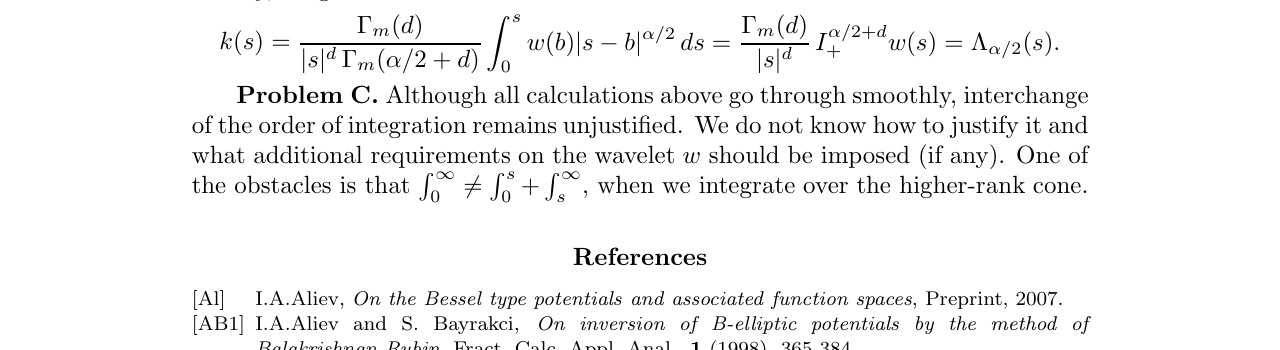
\includegraphics[width=0.96\textwidth]{figures/problem_c_crop.png}
\caption{The Fubini obstruction stated as Problem C, source PDF page 23.}
\end{figure}

\section{Verification, limitations, and novelty}

The proof was audited along eight focused routes: exact source scope;
comparison with the direct-wavelet predecessor \cite{oor}; the general
spectral reduction; necessity of the weighted criterion; the boundary-free
Cayley derivative; the matrix-beta constant; the $L^2$ domain and truncation;
and the Problem B/C scope distinction.  A symbolic checker verifies the first
$m=2$ Rodrigues identity and scalar numerical specializations; no computation
is proof-critical.

The most delicate review point is Lemma~\ref{lem:rodrigues}, specifically the
absence of boundary distributions under (7).  This is the standard safe
range of the determinant Riesz distribution and is stronger than needed for
some individual parameters.  The proof deliberately does not assert
pointwise convergence or an $L^p$ theorem for $p\neq2$.

Cheap run indexes, exact title/arXiv/problem searches, cone-heat-wavelet
keyword searches, and the full source of arXiv:math/0409100 were checked.  No
later exact answer was located through 2026-08-13.  The predecessor proves a
related direct multiscaled-wavelet theorem but assumes, for Riesz inversion,
a Fourier profile supported away from the rank-deficient boundary.  A
nonzero cone Laplace profile cannot satisfy that hypothesis.  Novelty remains
cautious because the present multiplier argument is philosophically close to
that predecessor and the Rodrigues family may exist in matrix-Laguerre
language.

\paragraph{Human-review recommendation.}
High-priority expert review.  Verify the Cayley/Riesz safe-range statement,
then check the scope judgment that an $L^2$ solution is a full answer to the
source's phrase ``$L_p$ or any other natural function space.''

\begin{thebibliography}{9}
\bibitem{source}
I.~A.~Aliev, B.~Rubin, S.~Sezer, and S.~B.~Uyhan,
\emph{Composite Wavelet Transforms: Applications and Perspectives},
arXiv:0711.1424v1 (2007); Contemp. Math. 464 (2008), 1--25.

\bibitem{oor}
G.~Ólafsson, E.~Ournycheva, and B.~Rubin,
\emph{Multiscaled wavelet transforms, ridgelet transforms, and Radon
transforms on the space of matrices},
arXiv:math/0409100; Appl. Comput. Harmon. Anal. 21 (2006), 182--203.

\bibitem{farautkoranyi}
J.~Faraut and A.~Korányi,
\emph{Analysis on Symmetric Cones}, Oxford Mathematical Monographs,
Clarendon Press, 1994.
\end{thebibliography}

\end{document}
